\documentclass[danish]{article}
\usepackage[T1]{fontenc}
%\usepackage[utf8]{inputenc}

\usepackage[danish]{babel}
%\usepackage[danish]{isodate}
\usepackage[dvipsnames,table]{xcolor}

\usepackage{ulem}
%https://mirrors.dotsrc.org/ctan/macros/luatex/latex/emoji/emoji-doc.pdf
%\usepackage{emoji}
\usepackage{amsmath,amsfonts,amssymb,amsthm}
\usepackage{multirow}
\usepackage{lilyglyphs} %https://www.ctan.org/pkg/lilyglyphs
\usepackage{boldline}
\usepackage{etoolbox}
\usepackage{xstring}
\usepackage{csquotes}
%\usepackage{datetime}
\usepackage{microtype}
%\usepackage{newspaper}
\usepackage{yfonts}  % used for the paper title font
\usepackage{fontspec}
%\usepackage{
%\date{\today}

%\SetPaperName{Solsikke Tidende}
%\SetPaperLocation{Santiago de Cali}
%\SetPaperSlogan{\clefG \hspace{0.15cm} \textbf{$Cipher_{Caesar}(_3)$} \hspace{0.15cm} \clefG}
%\SetPaperPrice{}

\DeclareFontFamily{LYG}{bigygoth}{}
\DeclareFontShape{LYG}{bigygoth}{m}{n}{<->s*[2.5]ygoth}{}

\setlength\topmargin{-48pt} 		% article default = -58pt
\setlength\headheight{0pt}  		% article default = 12pt
\setlength\headsep{34pt}		% article default = 25pt
\setlength\marginparwidth{-20pt}	% article default = 121pt
\setlength\textwidth{7.0in}		% article default = 418pt
\setlength\textheight{9.5in}		% article default = 296pt
\setlength\oddsidemargin{-30pt}



\def\papername{Solsikke Tidende}
\def\headername{Solsikke Tidende}   % because of the yfonts you may need both papername and headername
\def\paperlocation{København}
\def\musagsduhint{{\footnotesize \clefG} \hspace{0.15cm} \textbf{$Cipher_{Caesar}(4)$} \hspace{0.15cm} {\footnotesize \clefG}}
\newcommand\muzait{{\scriptsize\twoBeamedQuavers}\,}

\newcommand\muzaselection[3]{
  \paragraph{}
  {\fontfamily{lmr}\selectfont
  \textit{
    \muzait 
    {\Large\textbf{\StrLeft{#1}{1}}}\StrGobbleLeft{#1}{1}\, 
     \muzait} (#2) \\
  {\scriptsize
   \textit{
      \blockquote{#3}
    }
  }
}}

\def\paperprice{0 DKK}

\newcounter{volumeno}
\setcounter{volumeno}{65}
\newcounter{issueno}
\setcounter{issueno}{26}



\usepackage{times}
\usepackage{graphicx}
\usepackage{multicol}
\usepackage{picinpar}

\usepackage{lipsum}


%\colorlet{cfernando}{LightSteeleBlue3}
\definecolor{cfernando}{RGB}{38,40,74}
\definecolor{canna}{RGB}{164, 39, 168}
\definecolor{csune}{RGB}{125,21,21}
\definecolor{cother}{RGB}{103, 103, 152}


\newcommand\sayanna[1]{
  {\fontfamily{lmr}\selectfont \color{canna}{\textit{- #1}}}
}

\newcommand\sayfernando[1]{
  {\fontfamily{lmr}\selectfont \color{cfernando}{\textit{- #1}}}
}

\newcommand\saysune[1]{
  {\setmainfont{Ink Free} \color{csune}{\textit{- #1}}}
}

\newcommand\sayother[1]{
  {\fontfamily{lmr}\selectfont \color{cother}{\textit{- #1}}}
}



\newcommand\translatedfrom[1]{
 \begin{center}
  {\fontfamily{lmdh}\selectfont
  {\textit{oversat fra #1}}
  }
 \end{center}

}


\renewcommand{\maketitle}{
  \thispagestyle{empty}
  \vspace*{-40pt}
  \begin{center}
  \hfill
  {\textgoth
   {\huge 
     \usefont{LYG}{bigygoth}{m}{n} \papername
   }
  }\hfill%	
  \raisebox{12pt}{
   \textbf{
    \footnotesize 
    \paperlocation
   }
  }\\
  \vspace*{0.1in}
  \rule[0pt]{\textwidth}{0.5pt}\\
  {\small 
     Særudgave II: Chief Musical Officer
   } \hfill 
   \MakeUppercase{\small  13. december 2023} 
   \hfill {\small }\\
  \rule[6pt]{\textwidth}{1.2pt}
  \end{center}
  \pagestyle{plain}
}

\def\ps@plain{%
  \renewcommand\@oddfoot{}%					% empty recto footer
  \let\@evenfoot\@oddfoot						% empty verso footer
  \renewcommand\@evenhead
  {\parbox{\textwidth}{\vspace*{4pt}
  {\small VOL.\MakeUppercase{\roman{volumeno}}\ldots No.\arabic{issueno}}\hfill\normalfont\textbf{\headername}\quad\MakeUppercase{\textit\today}\hfill\textrm{\thepage}\\
  \rule{\textwidth}{0.5pt}
  \vspace*{12pt}}}%
  \let\@oddhead\@evenhead
}
		

\newcommand\headline[1]{
  {\fontfamily{lmdh}\selectfont
    \begin{center} #1\\ %
    \rule[3pt]{0.4\hsize}{0.5pt}\\ \end{center} \par
  }
}

\newcommand\byline[2]{
  {\fontfamily{lmdh}\selectfont
  \begin{center} #1 \\%
  {\footnotesize\bf af \MakeUppercase{#2}} \\ %
  \rule[3pt]{0.4\hsize}{0.5pt}\\ \end{center} \par
  }
}


\newcommand\closearticle{{\begin{center}\rule[6pt]{\hsize}{1pt}\vspace*{-16pt}
			\rule{\hsize}{0.5pt}\end{center}}}



\begin{document}

\begin{titlepage} % Suppresses headers and footers on the title page

	\raggedleft % Right align everything
	
	\vspace*{\baselineskip} % Whitespace at the top of the page


\begin{center}
  {\textgoth
   {\Huge 
     \usefont{LYG}{bigygoth}{m}{n} \papername
   }
  }	
\end{center}
\vspace{50px} 
	

\begin{center}
           \includegraphics[scale=2.2]{knojern-of-love}
\end{center}

%------------------------------------------------
%	Publisher
%------------------------------------------------

%{\large ~~\plogo} % Publisher and logo

\vspace{50px} 

          {
              \setmainfont{Ink Free} 
                   {\huge Særudgave II:}
                 \color{csune}{
                    {\huge
                        \textit{Chief Musical Officer}
                    }
                 }
           }



\vspace*{3\baselineskip} % Whitespace at the bottom of the page

\end{titlepage}



\maketitle
\fontfamily{phv}\selectfont

\begin{multicols}{2}
\byline{Just when I thought I was out...}{Fernándo Sanchez}
%\subsection*{Flugten fra Laksegade}

Kl. var 21:05 tirsdag den 12. december, da jeg stod af 500s med retning mod Glostrup st. Denne opgave var omtrent noget af det sidste jeg havde lyst til, efter at have brugt de sidste næsten 24 timer på at vaske op hos Price i Tivoli, men Anna havde ikke givet mig meget tid at løbe på: hvis jeg ville undgå at få uventet besøg af mine tidligere colombianske venner, skulle opgaven udføres til aften.\\
Jeg har efterhånden haft glæden af at besøge København en del gange, men jeg har aldrig begivet mig længere væk fra centrum end Vanløse, så jeg vidste ikke rigtigt hvad jeg kunne forvente mig af området. At dømme ud fra den store grå kolos der tonede frem i bussens forrude efterhånden som vi nærmede os mit stop, og rækken af mindre kolosser der lå som om Gud havde været ved at gøre klar til et spil 10 på stribe, inden han fuldstændigt havde glemt alt om området: ikke meget. Det gav et lille sug i maven da jeg stod af bussen, og bemærkede det 4 meter høje monument af et knojern der bød gæster til området velkommen. Jeg er ikke specielt overtroisk, og gør mig ikke så meget i at prøve at tyde tegn fra Gud, men det her virkede nu alligevel som om Gud prøvede at råbe mig an. \textit{``Så er det op med næverne makker!''}, og det i en situation hvor jeg egentlig mest havde lyst til at tage den næste bus ud af forstads-helvedet igen. Det er ikke fordi at jeg er sart, og CMO'en havde nok gjort sig mere end rigeligt fortjent til den skæbne der ventede ham men jeg kunne ikke lade være med at føle at jeg blev spillet som en brik i et spil som jeg ikke helt forstod. En brik med meget lav værdi, lod det til. Måske en halt bonde i et skakspil. Jeg måtte give Anna ret i at mandens opførsel var aparte, men var det virkeligt i en sådan grad at det var en trussel for hele organisationen?

\paragraph{}
Jeg bankede 3 gange hårdt på døren. Intet svar. Så 3 gange mere. Stadig intet svar. Jeg kunne se igennem dørspionen at der var lys derinde et sted, og hvor pokker skulle han ellers være henne? Vidste han at jeg kom? Gemte han sig? Hvorfor så ikke slukke lyset?\\
Jeg bankede på igen, men denne gang bankede jeg nærmere på 10 gange.\\

\saysune{HVEM ER DET DER BANKER PÅ MIN BRO? ha ha ha} lød det derinde fra.\\
Så blev døren åbnet af CMO'en der var iklædt shorts og bar overkrop, og så en hulens masse blæk på såvel overkrop som underkrop som pletvist rundt i ansigtet.\\

\saysune{JESPER! Næ det var satmne da en overraskelse. Jeg var lige ved at tattovere. Kom ind, kom ind for pokker. Hør, vil du også have en tattovering? Ååårh, vi kunne lave en Santa Muerte på dig, din slags er vilde med sådan noget. ``Puta pendejo, La Raza her, La Raza dér og Santa Muerte''... ha ha ha. Jeg kan ikke finde ud af at tegne, men jeg har transfer-papir! Ved du hvad, hvis du kan finde ud af at tegne, så kan vi begge to få én... Jeg kunne godt tænke mig en tattovering af Santa Muerte der byder op til dans på maven. Hvor vil du have din Santa Muerte?}\\
\sayfernando{Jeg er ikke kommet for at få en tattovering} sagde jeg tørt.\\
\saysune{Nå ja, det må du sgu da også selv om så... Men lad mig tage din jakke... Såådan ja... det var en stor dreng... ha ha ha...}\\
Idet han tog min jakke faldt pilleglasset med stryknin ud af jakkelommen og landede ret så åbenlyst på gulvet foran ham og nærmest skreg til omverdenen: \textit{``Her er jeg! Jeg er stryknin!''}, og jeg knækkede mine fingre og nakke for at gøre klar på den kamp der ville gå i gang om lidt.\\
\saysune{Hvad fanden er det dér Jesper? Har du taget stryknin med til mig? Det skulle du da ikke! Jeg har egentligt lovet mig selv at jeg ikke ville røre det stads i et halvt års tid... Min tolerance var simpelthen blevet for høj... Det ville have ruineret mig hvis jeg var fortsat... men nu hvor du alligevel har taget med: har du noget imod at jeg lige nupper en enkelt eller to?}\\
Det var ærligt talt ikke den reaktion jeg havde forventet, og jeg kan ikke huske om jeg nåede at formulere et svar inden han havde kørt 3 piller indenbords.\\

\saysune{For helvede, du må hellere stoppe mig inden jeg først rigtigt går ombord... så bliver der sgu ikke nogen til dig... ha ha ha... grib... Nå, du vil garanteret vildt gerne se lejligheden... Den er funktionsindrettet... Det ved du garanteret ikke hvad betyder... Vi er gode til sammensatte ord i Danmark... Det betyder at jeg nøje har sammensat inventaret efter dets funktion, så det passer lige præcis til mig. Kan du se den sorte kasse dér? Det hedder en X-Box... Det er et stykke elektronik der gør at man kan få tæv i raket-fodbold af 12-årige der sidder på den anden side af jorden... Det må altsammen være meget nyt for sådan én som dig... Det dér er en lænestol... Det er ligesom en taburet, bare meget bedre... Er du blevet tilbudt bolig i området? Sig mig, hvor har du egentligt min adresse fra?}\\

\sayfernando{Anna gav mig den}\\
\saysune{Oh...}\\

CMO'en havde indtil nu været stormflod af ord; som vandet fra en brast dæmning der oversvømmer den stakkel som vover at krydse dets vej, efter at have været indespærret i en lejlighed i forstaden for lang tid, men med ét var det som om hele hans væsen sænkede farten.\\

\saysune{Er du strapped?}\\
\sayfernando{Nej}\\
\saysune{Perfekt! Ser du Jesper, her i Danmark tror vi på nogle fyre der hedder Tor og Odin... Det er ligesom I har ham den flyvende fyr i skyerne og Sønnen på korset... Og når vi dør, har vi muligheden for at komme et sted hen der hedder Valhalla, og dér kæmper man med svær og økser hele dagen, og om aftenen bliver man sat sammen igen og spiser og drikker hvad hjertet begærer og så starter det hele forfra igen dagen efter, men det er slet ikke det bedste... Prøv at se her...}\\
Han trak sin telefon frem fra lommen af sine shorts, fandt nogle billeder frem og rakte mig telefonen.\\
\saysune{Det her, er Valkyrierne.. prøv at bladre videre til nummer 3... Nøøøj, hva?... Jeg håber at hende dér henter mig... Ser du, når vi dør, så kommer Valkyrierne og henter os og tager os med til Valhalla, og hvem ved hvad der kan ske af romantik på sådan en tur under stjernerne?}\\
Et drømmende blik gled henover hans øjne.
\saysune{Jeg ved teknisk set ikke om Valhalla er oppe eller nede... men der kan vel ikke være så meget romantik i at suse igennem jorden, vel? Lad os sige at det er oppe... Det må man selv bestemme... Men Jesper, alle de her herligheder tilfalder kun dem der dør tappert i kamp... vores regelsæt på det punkt kunne måske godt trænge til et eftersyn... jeg mener, er det ikke lidt unfair hvis man er mega-tapper hele sit liv, men så er der en snigskytte der napper én uden at man kan gøre modstand? Det er også ligemeget, for du har ikke en pistol... næh du! Du og jeg skal kæmpe til døden på gammeldags manér!}\\
\sayfernando{Så du ved hvorfor jeg er kommet?}\\
\saysune{Altså, jeg havde ikke lige forudset at hun ville sende dig, men det giver mening: du har... relevant erhvervs-erfaring ha ha... din relation til Anna er ikke tættere end at hun har ``Plausible Deniability''... Det giver mening}\\
\saysune{Jeg vidste at jeg ville ende her da jeg så resultatet af playoff-genereringen i lørdags}\\
\sayfernando{Playoffs...?}\\
\saysune{LOOOLS... Har hun ikke fortalt dig hvorfor hun har sendt dig?}\\
\sayfernando{Du er blevet... mærkelig...}\\
\saysune{Aaarhh ha ha ha ... Er det hvad hun fortalte dig? Din store idiot! Var du ikke på besøg i `18? Det her er sgu da den trætte udgave... ``vintage'' som man siger... }\\
\saysune{Undskyld! Idiot er et bum-ord. Det var ikke pænt af mig at kalde dig en idiot, men for helvede Jesper: det er jo i morgen at det helt store slag skal stå! Anna's darling: ``Juleshots'' vs. den absolutte BANGER ``The Season's Upon Us''! Det kunne have været en finale, og nu sker det i 1/8-dels finalen. Hun vil slet ikke kunne håndtere hvis jeg gjorde noget der fik ``Juleshots'' til at ryge ud i 1/8-dels finalen... hun er meget lidenskabelig på det punkt!}\\
\sayfernando{Og du har det OK med at jeg er blevet sendt herud for at... sikre et fair resultat i morgen? Du synes ikke at det virker en smule... drastisk?}\\
\saysune{Det ved jeg sgu ikke noget om ha ha... Vi skal jo allesammen den vej en dag, og bedre at det er dig og Anna end... ``de andre''}\\
\sayfernando{``De andre''?}\\
\saysune{Hell-divers, La Raza, ledelsen fra de andre dimensioner, ledelsen fra de andre finansielle institutter i Danmark. Der er nok at tage af}\\
\sayfernando{Hvorfor skulle de interessere sig for en musik-ansvarlig?}\\
\saysune{For helvede Jesper, du presser ikke ligefrem fartgrænsen i dag. Nå nå, nu skal jeg forklare dig det. Det her handler om meget mere end musik! Den der styrer den 3. dimension om 5 år, styrer FREMTIDEN! Kom med ind i træningssalen, så skal jeg piktogramme det for dig. Ud af den her dimension har vi kompetencer. Og her har vi leverancer. Men den nød som corporate ikke har kunne finde ud af at knække er, hvordan man opskalerer. Ser du, det at bygge software er ikke ligesom når I laver jeres pyramider... jeg mener, hvis man har dovne slaver når man bygger pyramider, så tager det måske bare dobbelt så lang tid, men hvis dem der bygger softwaren ikke har gnisten og viljen til at bevæge sig ind den jungle af kompleksitet som vi hver dag fører guerilla-krig i, så ender man med software som slet ikke kan bruges. Vi har i den 3. dimension knækket koden til at finde gejsten, men musikken er kun begyndelsen! Det er blot den udgravning som skal føre os ind til kernen... Ind til... KÆRLIGHEDEN! Kærligheden til kampen!}\\
Alt imens han fyrede denne svada af, forsøgte han efter bedste evne at afbillede hans syn på virkeligheden på en whiteboard-tavle der hang i hans træningssal. Om det var natten i køkkenet eller stormfloden af ord han havde kastet i hovedet på mig indenfor de sidste 15 minutter der havde udkørt mig er svært at sige, men jeg missede i hvert fald gode dele af den efterfølgende forklaring og at dømme ud fra den endelige tegning \ref{fig:madness} havde den del jeg gik glip af givet endnu mindre mening end den del jeg havde hørt.\\

\saysune{HØRER DU JESPER???}\\
\sayfernando{Hva'?}\\
\saysune{Skal vi gå ned og slås? Vi kan jo ikke være bekendt at kæmpe til døden heroppe... Jeg tror at dem nedenunder har en baby... Vi har jo ordnede forhold her i landet! Jeg foreslår at vi går op til  ``The Knojern of Love!''... Skønne rammer!}\\
Den bratte opvågning fik det absurde i hele situationen til at vælte ind over mig: hvis ikke jeg gjorde ét-eller-andet snart, ville jeg være nødt til at kæmpe til døden med denne galning foran det lokale vartegn, og så med ét, var det som om at Gud for 2. gang til aften rettede fokus imod min fortælling, for pludselig væltede CMO'en om i kraftige spasmer. 
\saysune{Uha da da... Nu sparker strykninen ind... ha ha ha... Uh! Den var god! Bare lige giv mig 2 minutter, så stopper spasmerne... det gør de altid... ha ha ha}\\
Jeg fornemmede at dette var mit cue til at tage benene på nakken, og jeg gjorde som jeg havde gjort så mange gange før på det seneste: løb som om Djævlen var lige i hælene på mig. På vej ned i opgangen kunne jeg høre CMO'en råbe efter mig:\\
\saysune{Kom tilbage din lort! BUM! Undskyld! Jeg har køkkenknive.. og escrima-stave... du må godt få den tunge af dem... det er nærmere en \textit{bâton}... HØRER DU JESPER??! EN BÂTON!}\\
\end{multicols}

\begin{figure}[h]
    \centering
    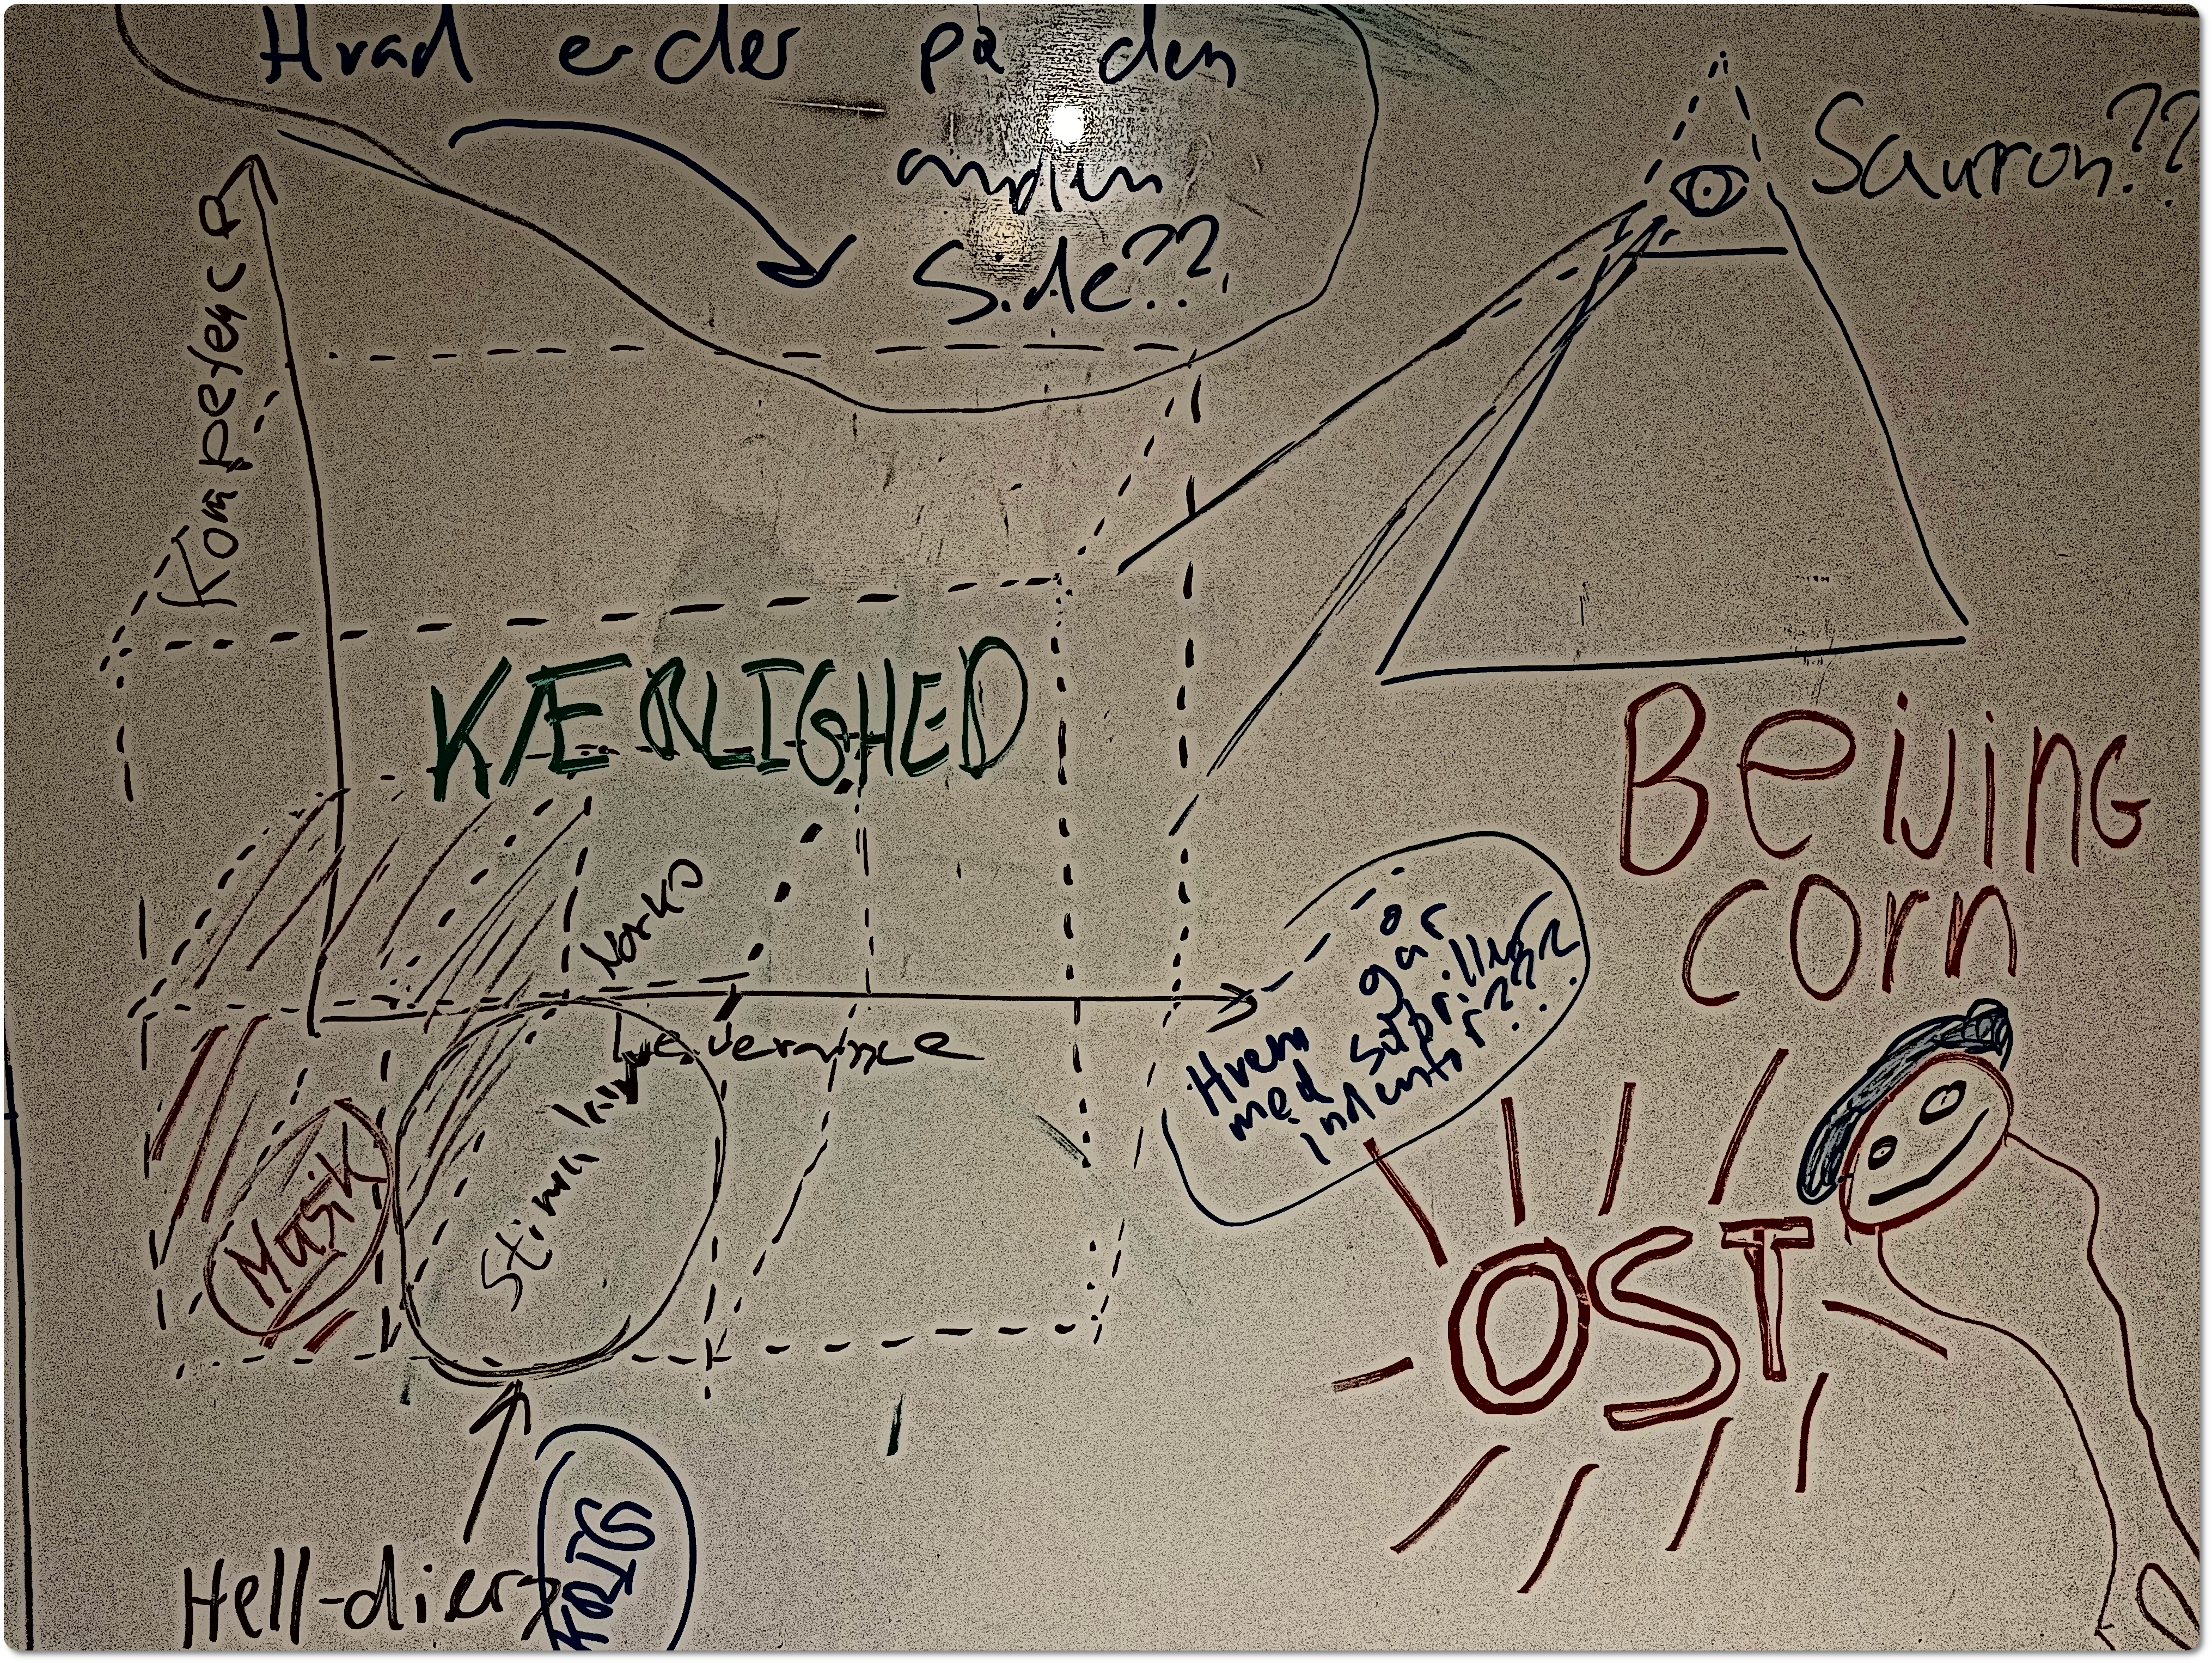
\includegraphics[width=1.00\textwidth]{madness.png}
    \caption{Jeg har ikke den fjerneste anelse om hvad \textit{The Eye of Sauron} har med sagen at gøre}
    \label{fig:madness}
\end{figure}


\end{document}